\section{Material und Methode}
\subsection{Teilnehmerauswahl}

In der vorliegenden wissenschaftlichen Arbeit wurde auf zwei divergierende Pools zur Rekrutierung der Teilnehmer zurückgegriffen. Der erste Rekrutierungspool umfasste diejenigen Individuen oder vermittelnden Kontakte\footnote{Ein vermittelnder Kontakt ist ein Kontakt, der einen potenziellen Studienteilnehmer aus seinem persönlichen Umfeld kontaktiert hat und diesen gefragt hat, ob er an der Studie teilnehmen möchte}, die eine Schulung für \textit{Schüler Online} besucht hatten. In diesen Schulungen wurde am Ende eine Folie präsentiert, die diese Studie vorstellte und um die Beteiligung der Anwesenden bat. Aus diesem Pool wurde die Sekretärin des Berufskollegs akquiriert.

Ein alternativer Weg zur Gewinnung von Teilnehmern war die Kaltakquise. Aus diesem Pool kamen alle weiteren Teilnehmer. Dabei wurden Schulen in zwei umliegenden Kreisen telefonisch kontaktiert und um ihre Teilnahme an der Studie gebeten. Aus Gründen der Vertraulichkeit und der Einhaltung von Verschwiegenheitsvereinbarungen ist es an dieser Stelle nicht möglich, konkrete Angaben zur Region zu machen.

Die Auswahl der Teilnehmer erfolgte basierend auf einer Reihe von Kriterien. Wesentlich war, dass die Teilnehmer in ihrem beruflichen Alltag das zu untersuchende Produkt sinnvoll einsetzen konnten - dies war ein entscheidendes Inklusionskriterium. Besonders geeignet waren daher Sekretariatsmitarbeiter, Schulverwaltungsassistenten und potenziell auch Schulleitungen. Als weiteres Inklusionskriterium war es erforderlich, dass die Teilnehmer aktiv in den genannten Berufen tätig und nicht in den Ruhestand getreten waren.

Im Gegenzug dazu wurden Auszubildende und Referendare von der Studie ausgeschlossen, da sie nur begrenzte Erfahrungen mit dem Tätigkeitsfeld der Software hatten. Dies stellte ein explizites Exklusionskriterium dar. Darüber hinaus spielten Faktoren wie Alter, Geschlecht, Berufserfahrung, ethnischer Hintergrund und sozioökonomischer Status der Teilnehmer bei der Rekrutierung keine Rolle.

Die Teilnahme an der Studie erforderte nur die Verfügbarkeit und die Bereitschaft der Teilnehmer, sich freiwillig zu engagieren. Es wurde darauf geachtet, dass keine Teilnahmeverpflichtungen, beispielsweise durch Vorgesetzte wie der Schulleitung, entstanden.

\subsection{Umgebungsbedingungen der Beobachtungen und Interviews}

Die Beobachtungen und Interviews wurden im Rahmen eines Feldtests abgehalten und fanden während der regulären Arbeitszeit an den gewohnten Arbeitsplätzen der Studienteilnehmer statt, um realistische Szenarien zu erzeugen. 

Die Durchführung der Interviews wurde während der Sommerferien terminiert. Es war von Bedeutung, den tatsächlichen Arbeitskontext der Teilnehmer einzubeziehen, um ein möglichst repräsentatives Bild ihrer Erfahrungen und Herausforderungen im Umgang mit dem untersuchten Produkt zu gewinnen.

\subsection{Erstellung des Fragebogens}

Die Formulierung des Fragebogens erfolgte durch eine Expertengruppe, die aufgrund ihrer beruflichen Rolle und Erfahrung eine hohe fachliche Expertise in Bezug auf die Anforderungen der zu untersuchenden Software besaßen. Diese Gruppe setzte sich zusammen aus Individuen, die im beruflichen Kontext die Anforderungen an die Software definierten und dokumentierten. Innerhalb dieser Gruppe gab es keinen Usability Experten, ledigliche einen Studenten, der das Fach \glqq Usability Engineering\grqq{} in seinem Studium belegte.

Um die Qualität und Eignung des Fragebogens zu gewährleisten, wurde dieser nach der Erstellung von einem Experten für Usability Engineering überprüft und auf seine inhaltliche Eignung hin bewertet.

Die Formulierung der Fragen folgte bestimmten Richtlinien: Sie sollten klar und verständlich sein und offen formuliert werden, um eine breite Palette von Antworten zu ermöglichen. Es war hier wichtig, dass der verwendete Sprachschatz laut Kruse den Kenntnissen eines Mitarbeitenden im Schulsekretariat entspricht.\cite{Kruse_2015} Dies gewährleistete, dass alle Teilnehmer die Fragen ohne zusätzliche Erläuterungen verstehen und beantworten können.

\subsection{Entwicklung von Aufgaben und Szenarien}
\begin{figure}[H]
    \caption{Einordnung der Aufgaben in den Gesamtkontext der Anwendung im Rahmen einer Beobachtungs- und Interviewstudie zur Bestimmung der Effektivität und Zufriedenstellung}
    \label{fig:EinordnungAufgaben}
    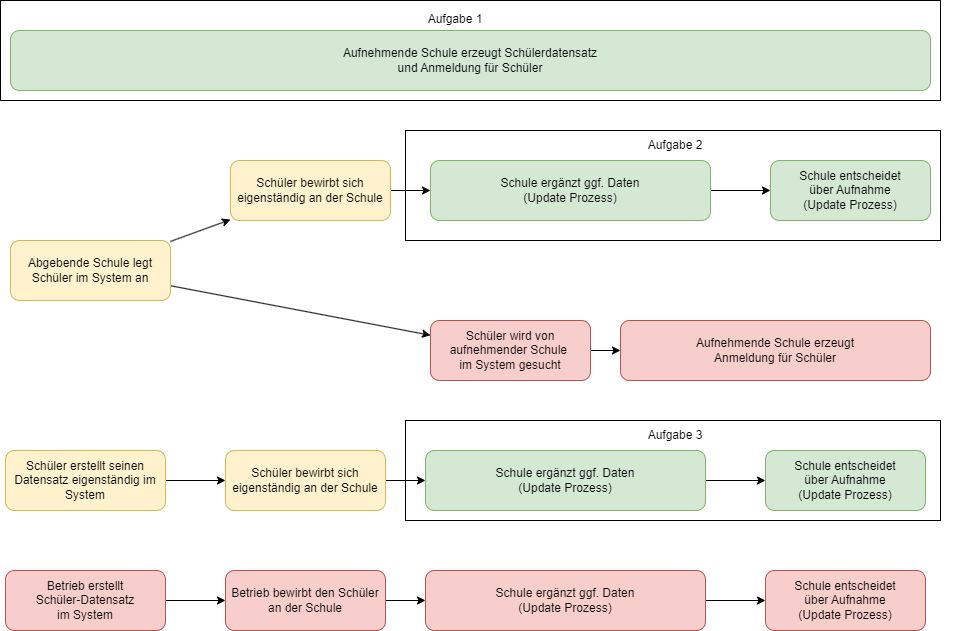
\includegraphics[width=\textwidth]{einordnung-der-aufgaben-in-kontext}
\end{figure}

Für die Durchführung des Feldtests wurden drei spezifische Aufgaben im System entwickelt, die die Teilnehmer während ihrer normalen Arbeitszeit bewältigen sollten. Dabei wurde darauf geachtet, dass die individuellen  Voraussetzungen für die jeweilige Schule gegeben waren, einschließlich  vorhandener Bildungsangebote an der jeweiligen Schule. Die konkreten Aufgaben lauteten wie folgt:

\begin{itemize}
\item Aufgabe 1: \glqq Erstellen Sie bitte für dieses Anmeldeformular von \textit{Max Müller} eine Bewerbung an Ihrer Schule.\grqq{} (Ein Musterexemplar eines solchen Formulars ist Anhang 1 zu entnehmen. Aufgabe 1 macht bisher rund 3,6\% aller erfassten Anmeldungen aus)
\item Aufgabe 2: \glqq Bearbeiten Sie bitte die Bewerbung von \textit{Lotta Meier} nach eigenem Ermessen.\grqq{}  Dieser fiktive Datensatz war so gestaltet, dass die Bewerbung entweder von einer abgebenden Schule oder von der Gemeinde gestellt wurde. Aufgabe 2 macht bisher rund 49,2\% aller erfassten Anmeldungen aus.
\item Aufgabe 3: \glqq Bearbeiten Sie bitte die Bewerbung von \textit{Konrad Schulz} nach eigenem Ermessen.\grqq{}  Bei diesem fiktiven Datensatz wurde die Bewerbung von den Eltern des Schülers eingereicht. Aufgabe 3 macht bisher rund 23,3\% aller erfassten Anmeldungen aus.\footnote{Die Datenquelle der Anteile sind interne Auswertungen des krz.}
\end{itemize}

Andere Anmeldearten sind nicht Gegenstand dieser Untersuchung, da sie zu umfangreich nachzustellen wären. Eine Visualisierung der drei Aufgaben inklusive ihres Kontextes sind in Abbildung \ref{fig:EinordnungAufgaben} ersichtlich. Die rot markierten Aktivitäten werden nicht untersucht. Gelb Markiertes sind vorbereitete Aktivitäten, welche Voraussetzung für die grün markierten zu untersuchenden Aufgabenaktivitäten sind. 

\begin{figure}[H]
    \caption{Übersicht der Aufgabenkonstellationen, gruppiert nach Schulstufe im Rahmen einer Beobachtungs- und Interviewstudie zur Bestimmung der Effektivität und Zufriedenstellung}
    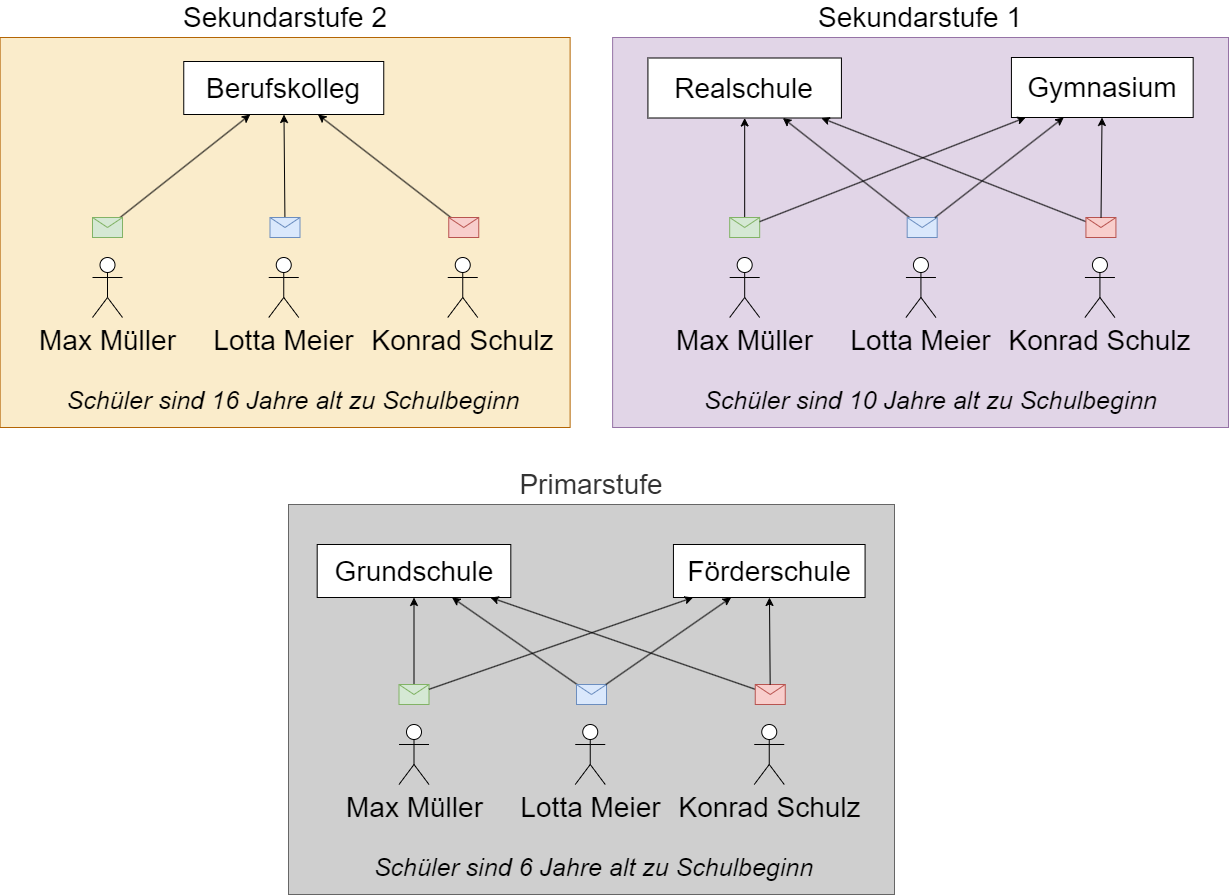
\includegraphics[width=\textwidth]{konstellationenv3}
\end{figure}

%\begin{figure}[H]
    %\centering
    %\caption{Musteranmeldeformular von der fiktiven Person Max Müller}
    %\begin{adjustbox}{width=\linewidth, center}
        %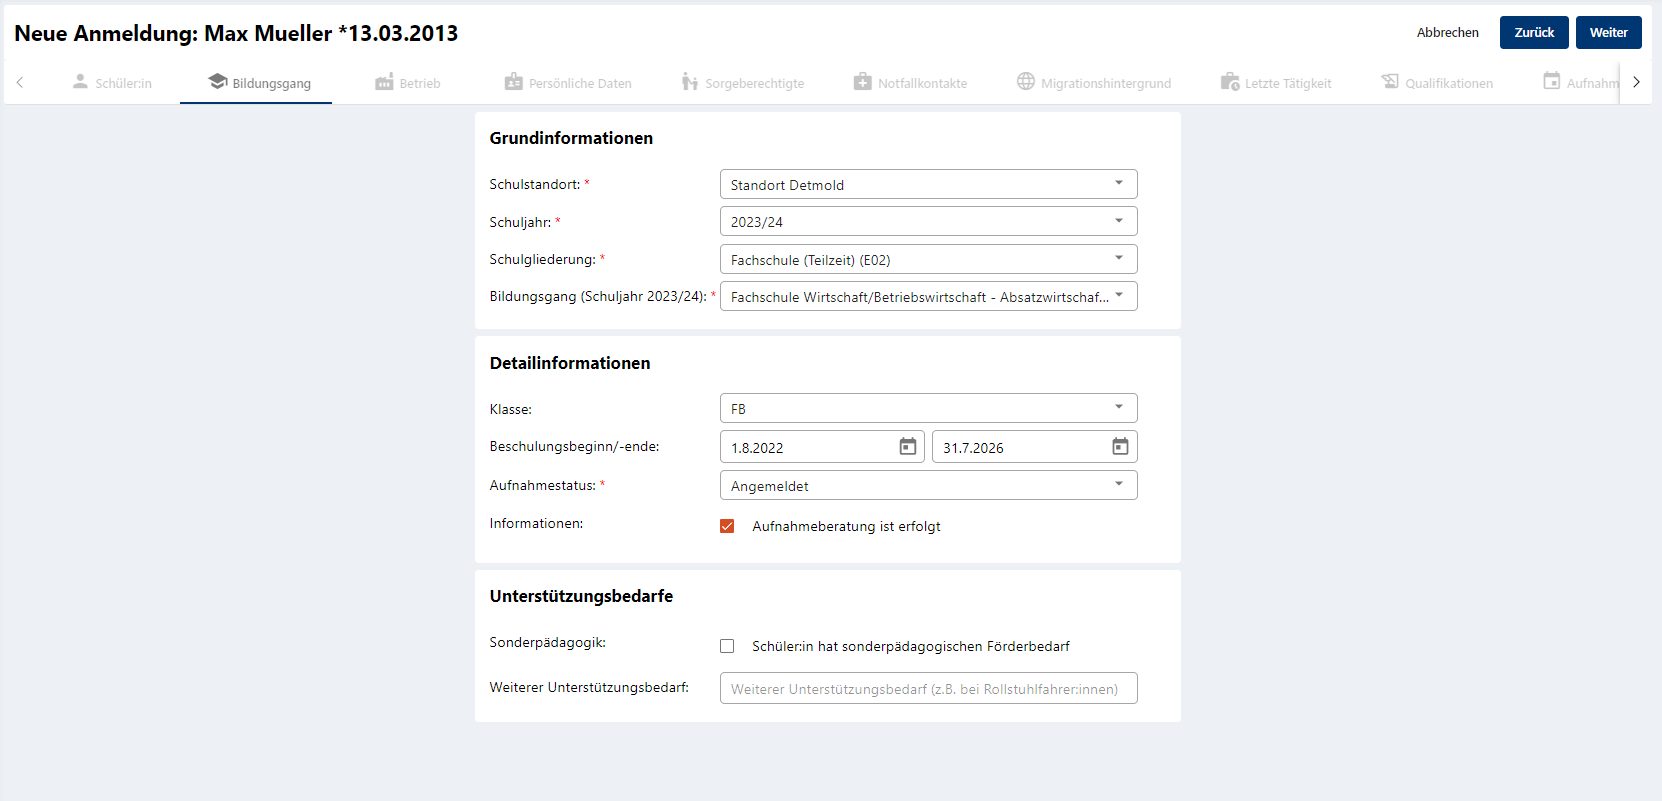
\includegraphics{bildungsgang}
    %\end{adjustbox}
%\end{figure}

Um den Realitätsbezug zu gewährleisten, unterschieden sich die Datensätze je nach Schule, insbesondere in Bezug auf das Geburtsjahr, das an die jeweilige Schulstufe angepasst wurde. So wurde für Bewerbungen an der Primarstufe das Geburtsdatum so gewählt, dass das Schulkind zum Zeitpunkt des ersten Schultages 6 Jahre alt wäre. Im Falle einer Bewerbung für die Sekundarstufe 1 war das Schulkind 10 Jahre und für die Sekundarstufe 2 entsprechend 16 Jahre alt.
Hierzu wurden so genannte Anmeldeformulare der jeweiligen Schule verwendet, die mit Ausnahme des Geburtsdatums und des zu besuchenden Bildungsgangs mit identischen Inhalten ausgefüllt wurden (s. Abbildung 1).

Zu beachten ist, dass alle Datensätze fiktiv waren, um etwaige Probleme hinsichtlich der Vertraulichkeit zu vermeiden. Dies wurde den Teilnehmern vor Beginn der Aufgaben explizit mitgeteilt.

\subsection{Bereitstellung des Fragebogens}

Im Vorfeld der Untersuchung wurde der Fragebogen den Studienteilnehmern nicht vorab zur Verfügung gestellt. In den initialen Telefongesprächen wurde jedem Teilnehmer ausdrücklich mitgeteilt, dass keine spezielle Vorbereitung für die Teilnahme an der Studie erforderlich sei. Die Software und der Zweck der Studie wurde jedem Teilnehmer in diesem Zuge ebenfalls kurz dargelegt.

Darüber hinaus wurden in diesen Gesprächen die Software \textit{Schüler Online} und der Zweck der Studie den Teilnehmern ausführlich erläutert. Dies gewährleistete, dass jeder Teilnehmer über den Kontext und die Ziele der Studie informiert war und eine Vorstellung von dem hatte, was von ihm oder ihr erwartet wurde.

\subsection{Rollenverteilung während der Studie}

Während der Durchführung der Studie gab es zwei Hauptrollen innerhalb des Forschungsteams: den Interviewer und den Schreiber. Der Interviewer, der die Software mehrere Jahre mitentwickelt hat, war mit den funktionalen Aspekten des Systems gut vertraut, hatte jedoch keine umfangreichen praktischen Erfahrungen hinsichtlich Interviewtechniken. Diese Rolle wurde durch eine Person besetzt, deren Aufgabe es war, die Teilnehmer durch die Aufgaben zu leiten und die Diskussion während des Interviews zu lenken.

Die Rolle des Schreibers wurde durch zwei Personen wahrgenommen, die sich abwechselten. Schreiber A nahm an den Interviews 1 und 4 teil, während Schreiber B an den Interviews 2, 3 und 5 präsent war. Beide Schreiber hatten grundlegende Kenntnisse der Software, die sie während des ersten Jahres ihrer Beteiligung an der Entwicklung der Software erworben hatten.

Die Hauptaufgabe der Schreiber war es, während der Interviews Notizen zu machen und die Reaktionen der Teilnehmer sowie relevante Beobachtungen zu dokumentieren. 

\subsection{Durchführung der Studie}

Die Implementierung der Studie wurde vor Ort in den Schulen durchgeführt. Der Interviewer und der Schreiber trafen sich persönlich mit den Teilnehmern. Beide stellten sich kurz vor und erläuterten den Zweck der zu untersuchenden Software.

Für die Interviews suchten sie sich innerhalb des Raums einen Ort aus, von dem aus sie sowohl den Monitor als auch den Probanden gut beobachten konnten. Während des Interviews stellte der Interviewer sowohl die Fragen aus dem Fragebogen als auch zusätzliche klärende Fragen. Der Notierer hingegen konzentrierte sich hauptsächlich darauf, die Antworten und Beobachtungen zu dokumentieren.

Die Beobachtung der Aufgabenbearbeitung und des Verhaltens der Teilnehmer war sowohl dem Interviewer als auch dem Notierer zugeordnet. Um ein realistisches Szenario zu gewährleisten, wurden keine fachlichen Rückfragen der Studienteilnehmer beantwortet - sie mussten sich, ähnlich wie in einer realen Arbeitsumgebung, auf die Dokumentation und ihre eigenen Ressourcen verlassen.

Den Teilnehmern wurde versichert, dass das Ziel der Studie war, die Software und nicht den Anwender zu testen. Das Interview und die Beobachtung fanden gleichzeitig statt und dauerten zwischen einer und drei Stunden.

Die Teilnehmer agierten entsprechend des \textit{Meister-Schüler-Modells} in der Rolle des Meisters, von denen der Schüler (Interviewer) lernen kann. Sie wurden dementsprechend nicht in ihren Ansichten korrigiert. %todo: Quelle

Um in dieser Ausarbeitung die Antworten und Beobachtungen zuordenbar zu machen, sind die Resultate der Sekretärinnen des Gymnasiums (1), der Realschule (2), der Förderschule (3), der Grundschule (4) und des Berufskollegs (5) konsequent und analog zu ihrer Indexziffer den Anhängen 2.1 bis 2.5 zugeordnet.

In der ersten Durchführung mit dem Gymnasium (1) gab es die Besonderheit, dass  in Anlehnung an die Empfehlung des Leitfaden Usability ein erfahrener Requirements Engineer (der Product Owner der Software) mittels Anruf zugeschaltet wurde, der \glqq in Form einer Supervision die Gesprächssituation beobachtet, bewertet und anschließend mit dem Beobachteten [besprochen hat]\grqq{}\cite{dakks}.

In drei Fällen (Gymnasium (1), Realschule (2) und zeitweise bei der Förderschule(3)) waren bei der Durchführung der Interviews zwei Mitarbeiter vonseiten der Studienteilnehmer anwesend. Es wurde die Entscheidung getroffen, das Interview nur mit dem vorab rekrutierten Teilnehmer durchzuführen. Kommentare und Diskussionen zwischen den Mitarbeitern waren jedoch zulässig, um ein realistischeres Szenario zu belassen. Die gesammelten Daten wurden ausschließlich aus den Ansichten, Antworten und Beobachtungen des Interviewpartners erfasst, nicht von dem weiteren Mitarbeiter. Die Interviews wurden direkt in Microsoft Word dokumentiert. Es wurden keine Audio- oder Filmaufnahmen erstellt.

\subsection{Nachbereitung und Auswertung der Studie}

Unmittelbar nach Abschluss der Interviews wurde eine erste Nachbearbeitung der gesammelten Daten durchgeführt. Hierbei wurden unklare oder zu kurz formulierte Notizen präzisiert und ausführlicher beschrieben. Es ist wichtig zu betonen, dass diese Nachbearbeitung nur für Einträge vorgenommen wurde, bei denen eine eindeutige Interpretation möglich war. Bei Notizen, bei denen das Potenzial für Fehlinterpretationen bestand oder die im Nachhinein unklar blieben, wurden keine Änderungen vorgenommen. Sie wurden in ihrer ursprünglichen Form beibehalten, um die Möglichkeit von Missverständnissen zu minimieren.

Für die Auswertung der gesammelten Daten wurden keine speziellen Analysetools oder ähnliche Instrumente verwendet. Die Auswertung erfolgte lediglich bei den Notizen, die unmissverständlich waren und bei denen man keine Fehlinterpretationen beim Ausformulieren machen konnte. Bei Punkten, die potenziell fehlinterpretiert werden konnten oder im Nachhinein unklar waren, wurden keine Ausformulierungen durchgeführt, sondern die Notiz so belassen wie sie mitgeschrieben wurde. Verständnis der Benutzererfahrungen und -bedürfnisse zu gewinnen.

%todo: Die Ergebnisse der unterschiedlichen Schulen wurden jedoch händisch miteinander auf Gemeinsamkeiten und Kontroversen verglichen. 


\subsection{Materialien und Ressourcen}

Für die Durchführung der Studie war vonseiten der Teilnehmer lediglich ein Computer mit Internetzugang erforderlich, um den Zugriff auf die Anwendung zu ermöglichen. Darüber hinaus war kein zusätzliches Material notwendig.
Vonseiten der Moderation wurden ein Laptop für Notizen und der ausgearbeitete Fragebogen sowie die Anmeldeformulare verwendet

%  Ethik: Welche ethischen Gesichtspunkte wurden bei der Durchführung des Interviews berücksichtigt, z.B. in Bezug auf Datenschutz oder Anonymität?
 
 
% In diesem Kapitel solltest du die Methoden und Techniken, die du zur Durchführung deiner Projektarbeit verwendest, beschreiben und begründen. Hier sollten auch die Einzelheiten zur Durchführung des leitfadengestützten Interviews enthalten sein.
% Für das leitfadengestützte Experteninterview solltest du in der Methodik deiner Projektarbeit den Ablauf und die Durchführung des Interviews beschreiben. Hierbei sollst du beispielsweise folgende Punkte erwähnen:
% Teilnehmer: Wer wurde für das Interview ausgewählt und warum? Wie viele Experten wurden befragt? 

% material
% Wie haben wir den Fragebogen erstellt? 
% Schulleiter zeigt nochmal weitere Aspekte auf
% Offene Fragen gemacht => Warum offene Fragen
% induktives vorgehen
% ich habe jedes Sekretärin vorher telefonisch gesprochen

% Fragebogen ist delegiert ans Team und ein Zwischenergebnis. Ist ein Ergebnis eines Expertenteams für dieses Programm
% Experten sind Material


% ggf. der fixierte Nutzungskontex 